
Uma \gls{bn} provê uma representação compacta de distribuições de probabilidades grandes demais para lidar usando especificações tradicionais e provê um método sistemático e localizado para incorporar informação probabilística sobre uma dada situação.

Uma BN é um \gls{dag} que representa uma função de distribuição de probabilidades conjunta de variáveis que modelam certo domínio de conhecimento. Ela é constituída de uma \gls{dag}, de variáveis aleatórias (também chamadas de nós da rede), arcos direcionados da variável pai para a variável filha e uma \gls{cpt} associada a cada variável.
\begin{figure}[H]
	\centering
	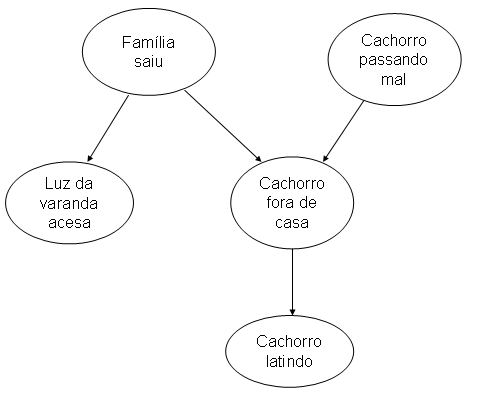
\includegraphics[width = 300px]{figuras/BN1}
	\caption[Exemplo family-out]{Exemplo family-out}
	\label{fig:familyBN}
\end{figure}

Nesse exemplo, suponhamos que se queira determinar se a família está em casa ou se ela saiu. Pelo grafo, podemos perceber que o fato de a luz da varanda estar acesa e de o cachorro estar fora de casa são indícios de que a família tenha saído. 

\section{Definição Formal}
Considere a \gls{bn} contendo $n$ nós, $X_1$ até $X_n$, tomados nesta ordem. Uma instanciação da distribuição disjunta de probabilidade é representada por $P(X_1 = x_1, X_2 = x_2, ... , X_n = x_n)$, ou de forma compacta $P(x_1, x_2, ..., x_n)$. A \textbf{regra da cadeia} nos permite fatorar probabilidades disjuntas como:
\begin{equation}
	P(x_1, x_2, ..., x_n) = P(x_1)P(x_2|x_1)...P(x_n|x_1,..,x_{n-1})\\
	= \prod_{i}^{}P(x_i|x_1,...,x_{i-1})
\end{equation}
No entanto, a estrutura de uma \gls{bn} implica que o valor de um nó em particular é condicionado apenas aos valores dos nós pais, o que reduz a equação acima à:
\begin{equation}\label{eq:pearl}
P(x_1, x_2, ..., x_n) = \prod_i P(x_i|pa_i)
\end{equation}
Onde $pa_i$ são os nós pais de $x_i$

\section{D-separation}
Segundo Cheng\cite{cheng02} Uma rede bayesiana pode ser vista como um sistema de rede de canais de informação, onde cada não é uma válvula que está aberta ou fechada e as válvulas são conectadas por canais de informação ruidosos (arestas). O fluxo de informação pode passar por um válvula aberta, mas não por uma válvula fechada. Quando todas as válvulas sobre um caminho entre dois não estão abertas, diz-se que este caminho é aberto. Se qualquer válvula no caminho está fechada, diz-se que o caminho é fechado.

Formalmente um caminho c é dito ser d-separado (ou bloqueado) por um conjunto de nós \textbf{Z} se e somente se:
\begin{itemize}
	\item c contem uma cadeia i $\rightarrow$ m $\rightarrow$ j ou uma divergência i $\leftarrow$ m $\rightarrow$ j tal que o nó do meio m está em \textbf{Z};
	\item c contem uma convergência (ou colisor) i $\rightarrow$ m $\leftarrow$ j tal que o nó do meio não está em $\textbf{Z}$ e nenhum descendente de m está em $\textbf{Z}$
\end{itemize}

O conjunto \textbf{Z} d-separa \textbf{X} de \textbf{Y} se e somente se, \textbf{Z} bloqueia todos os caminhos de nós em \textbf{X} para nós em \textbf{Y}.

Se um caminho satisfaz a condição acima, diz-se que ele é bloqueado; caso contrário ele é ativado por \textbf{Z}. Na figura \ref{fig:d-sep} $X$ = {2} e $Y$ = {3} são d-separados por Z = {1}; o caminho 2 $\leftarrow$ 1 $\rightarrow$ 3 é bloqueado por 1 $\in$ \textbf{Z}.
\begin{figure}[H]
	\centering
	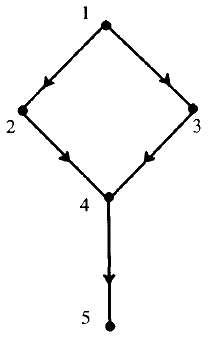
\includegraphics{figuras/d-separation}
	\caption[Exemplo D-separation]{Um \gls{dag} demostrando d-separation; o nó 1 bloqueia o caminho 2-1-3, enquanto o nó 5 ativa o caminho 2-4-3 (retirado de \cite{pearl88})}
	\label{fig:d-sep}
\end{figure}

Em 1988 Pearl prova que os conjuntos \textbf{X} e \textbf{Y} são d-separados por \textbf{Z} em \gls{dag} se e somente se \textbf{X} é independente de \textbf{Y} condicionado a \textbf{Z} em toda distribuição compatível com G.

Em outras palavras $(\textbf{X} \perp \textbf{Y}|\textbf{Z})_G \Leftrightarrow (\textbf{X}\perp\textbf{Y}|\textbf{Z})_P$, onde $(\textbf{X}\perp\textbf{Y}|\textbf{Z})_G$ significa que \textbf{X} é d-separado de \textbf{Y} dado \textbf{Z} em um grafo G, e $(\textbf{X}\perp \textbf{Y}|\textbf{Z})_P$ é a independência estatística como discutido na sessão anterior.

\section{M-separation}
Um teste alternativo para d-separação foi proposto por Lauritzen \cite{lauritzen90}, baseado na noção de grafos ancestrais e foi chamada de m-separação (separação moralizada) por Silva e Ladeira \cite{daSL02}.
\begin{itemize}
	\item Exclua de G todos os nós exceto aquele em anc(\textbf{X} $\cup$ \textbf{Y} $\cup$ \textbf{Z});
	\item Conecte por uma aresta todo par de nós que possuam filho em comum (moralização);
	\item Remova todas orientações dos arcos
\end{itemize}
Então $(\textbf{X} \perp \textbf{Y}|\textbf{Z})_G$ se e somente se, \textbf{Z} intercepta todos os caminhos entre \textbf{X} e \textbf{Y} no grafo não orientado resultante. Isto é, se removendo \textbf{X}, \textbf{Y} e \textbf{Z} ficam desconectados, então \textbf{X} e \textbf{Y}são condicionalmente independentes dado \textbf{Z}, caso contrário \textbf{X} e \textbf{Y} são dependentes dado Z. Onde \textbf(anc(W)) contém os nós de W e todos seus ancestrais.

O Benefício de m-separação sobre a d-separação é o fato de ser um processo algorítmico e portanto fácil de se implementar.
